\begin{figure*}
\begin{centering}
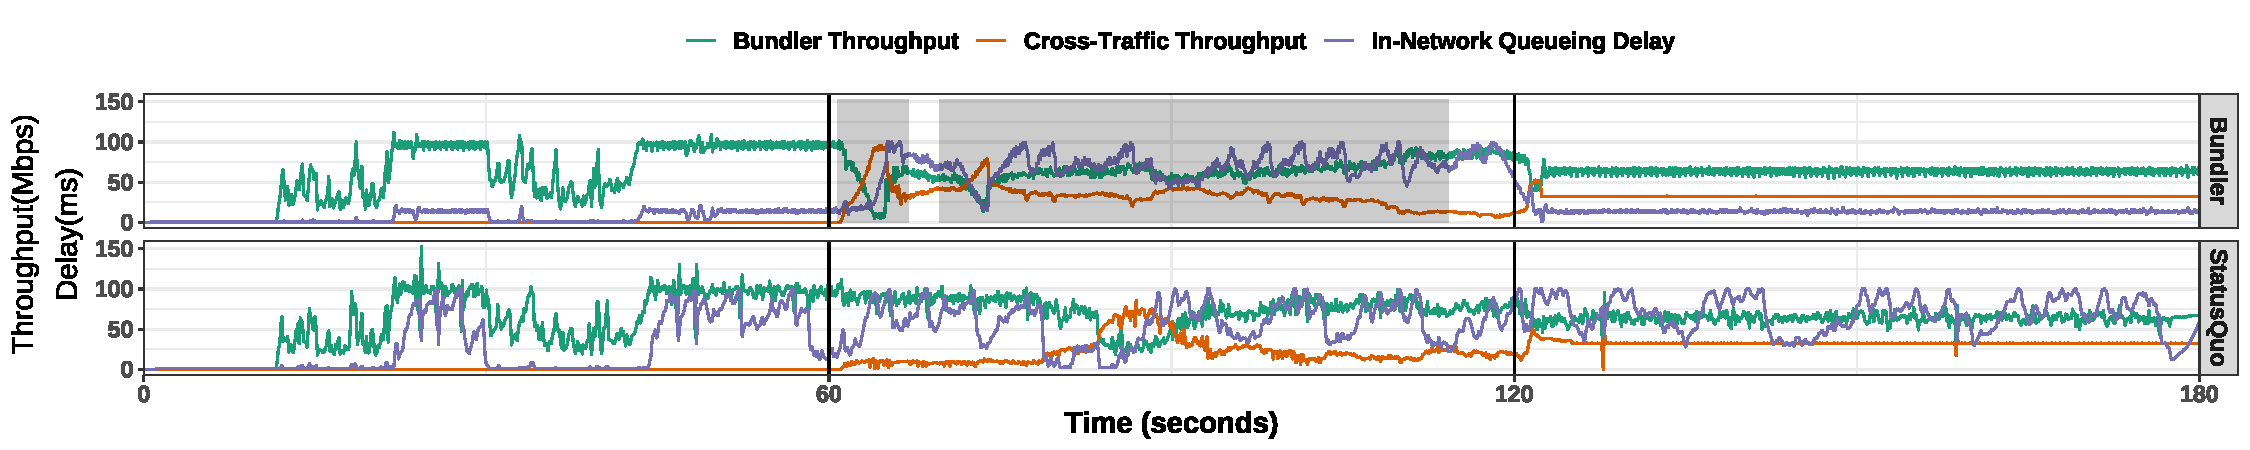
\includegraphics[width=\textwidth]{big_exp/mm}
\end{centering}
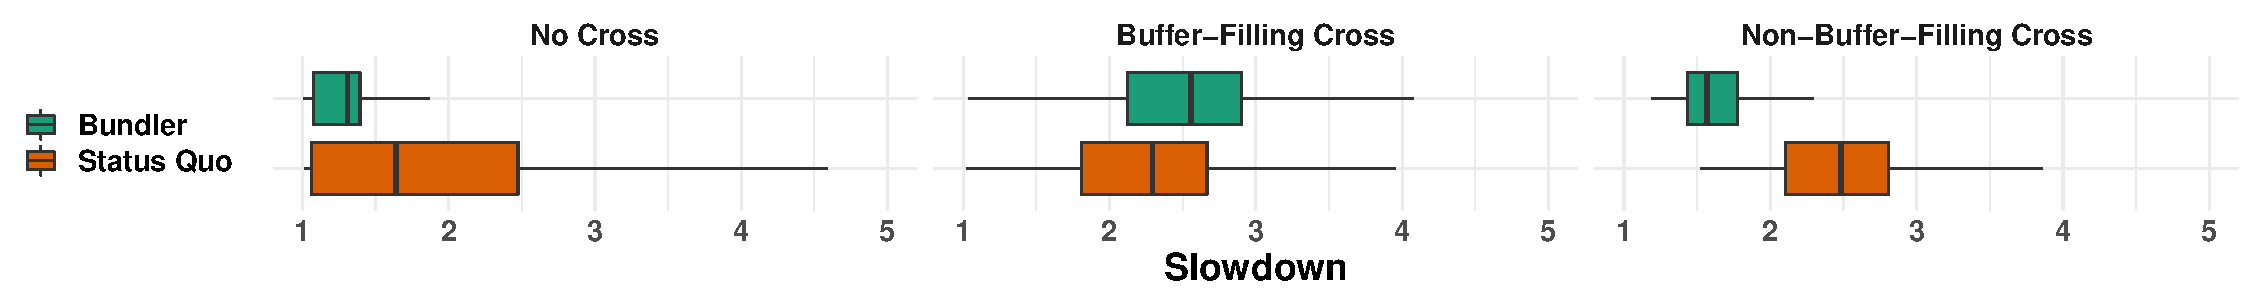
\includegraphics[width=0.95\textwidth]{big_exp/big_exp_41/big_exp_fct}
\caption{\name's scheduling ability depends on the characteristics of the cross traffic over time. In this experiment, there are 3 periods: from 0 to 60 sec., there is no competing traffic, from 60 to 120 sec. there is buffer-filling cross traffic, and from 120 to 180 sec. there is non-buffer-filling cross traffic. During the period with buffer-filling cross traffic, \name detects its presence and reverts to status-quo performance. The shaded region in the \name graph shows the output of the cross-traffic detector.}\label{fig:eval:bigexp}
\end{figure*}